\chapter{Implementace: Vývoj v App Engine}

\section{Výběr cloudu}
Pro praktickou ukázku a prověření implementace jsem vybral cloud App Engine od společnosti Google. Nejdůležitějším důvodem pro mne byla možnost nahrát plnohodnotnou aplikaci bez nutnosti vynaložení jakýchkoliv nákladů na hosting. Nastavené kvóty od kterých je nutné platit jsou vysoké (odpovídají několika stovkám tisíců požadavků za den) a stále se postupně zvyšují. Je tedy možné s tímto cloudem libovolně experimentovat a nahrávat různé testovací aplikace. Mnoho Java vývojářů hledá pro svoje malé aplikace hosting, kde by nemuseli platit, anebo mohli nahrát více aplikací. To je ale problém webového Java světa. Server počítá pouze s jedinou aplikací a je často nutné si pamatovat prostředky a další zdroje v rámci aplikace mezi požadavky. Javovský server tak počítá s tím, že si alokuje většinu dostupné paměti systému. Výhodou je, že nemusíme při každém požadavku vytvářet nové spojení do databáze a k ostatním prostředkům. Naproti tomu u skriptovací jazyků (jako například \verb|PHP| nebo \verb|Python|), se při každém požadavku provede celý kód znovu. Na serveru tak může běžet několik aplikací a zároveň se neovlivňují. V praxi se toho běžně využívá a proto je možné provozovat velké množství takovýchto aplikací na jediném hostingu. App Engine nám umožňuje stejný princip pro Javu, běh více aplikací na stejném hardware. Cena za tuto možnost je nutnost uvolnění zdrojů z nepoužívaných aplikací, aby nezabíraly místo ostatním. To App Engine sám hlídá a po určité době neaktivity aplikaci odstaví a nahraje aktivní.

\section{Aplikace}
Cílem této bakalářské práce je ověřit možnosti a omezení škálovatelných aplikací. Nejdůležitějším hlediskem je celková rychlost a odezva aplikace v závislosti na počtu souběžných požadavků. Tedy jak bude aplikace a celý cloud reagovat na zvýšený nápor požadavků, jak se s tím cloud vyrovná a zda bude služba stále použitelná. Také jsem se zaměřil na rychlost čtení a ukládání do Datastore. Pokud je klasická aplikace vystavena vysoké zátěži, je ve většině případů právě databáze úzkým hrdlem (takzvaný \emph{bottleneck}) a přestává stíhat zpracovávat požadavky jako první. 

Kromě ověření rychlosti a škálovatelnosi bylo také cílem vytvořit rozsáhlejší aplikaci a vyzkoušet všechny úskalí, které nám platforma App Engine staví do cesty. To znamená implementace běžných požadavků na aplikace, například M:N\footnote{Many-to-Many - druh relace, kde více entit může být spojeno s více entitami (M:N), v relačních databázích je pro propojení použita spojovací tabulka} relace mezi entitami, zamykání dat proti přepsání a další požadavky, které jsou na aplikace běžně kladeny. Po vytvoření tohoto základu a překonání všech zádrhelů již bude jednoduché takovouto aplikaci upravit pro jiné požadavky, anebo rozšířit o nové funkce.

Jako nejvhodnější řešení pro vyzkoušení implementace jsem vybral jednoduchý systém pro správu obsahu (CMS - Content Management System). Můžeme si tak vytvořit webovou  stránku s plnou administrací, tedy s možností přidávání, úpravy a mazání stránek. Ke každé stránce můžeme přidat šablonu. Mimo samotných stránek lze přidávat, upravovat a mazat i novinky. Jedná se o kratší zprávy, pro které je zbytečné vytvářet samostatnou stránku. Ke každé stránce lze také přiřadit štítek (tag), tato možnost nahrazuje kategorie. Výhodou oproti kategoriím, kde může být jeden článek pouze v jedné kategorii je, že článek může být označen více štítky a zároveň jeden štítek může být přiřazen k více článkům. Z těchto údajů pak můžeme generovat takzvané \emph{tag cloudy} (oblaky štítků)\footnote{http://en.wikipedia.org/wiki/Tag\_cloud}, kde velikost štítku určuje jeho význam, Čím více článků štítek označuje, tím je důležitější a výraznější. Z hlediska implementace se jedná o vazbu M:N, která se v NoSQL databázích musí implementovat složitěji než v relačních a bylo potřeba vymyslet vyhovující řešení.

\section{Výběr frameworku: Slim3}
Před započetím práce jsem zjišťoval, které knihovny a frameworky\footnote{Framework je ucelený soubor knihoven a kódu pomáhající vytvořit aplikaci} bych mohl použít na ulehčení práce. Kvůli omezením nejsou podporovány všechny knihovny a některé potřebují speciální úpravy anebo nastavení. Další nevýhodou je, že čím je náš kód rozsáhleší, tím déle bude trvat načítání pokaždé, když bude App Engine nahrávat aplikaci do aktivního stavu. Tímto jsem eliminoval velké frameworky jako jsou Spring\footnote{Spring Framework - http://www.springsource.org/} a Seam\footnote{Seam Framework - http://seamframework.org/}. Poté jsem hledal mezi menšími, ale žádný nevyhovoval úplně potřebám App Engine. Bohužel je tento cloud relativně mladý a tak pro něj neexistují frameworky, anebo jsou málo známé. Uvažoval jsem tedy že použiji přímočaré řešení pomocí servletů a naprogramuji aplikaci od základů. Naštěstí jsem ale náhodou narazil na framework Slim3\footnote{Slim3 - http://sites.google.com/site/slim3appengine/} určený přesně pro potřeby App Engine.

Slim3 je MVC\footnote{Model View Controller - http://en.wikipedia.org/wiki/Model-view-controller}
framework optimalizovaný pro App Engine, přináší rozšíření i jednodušší práci s Datastore API a další vylepšení. Jeho hlavní koncepty jsou: \emph{simple} (jednoduchý) a \emph{less is more} (méně je více), tedy že jednoduchost a srozumitelnost vedou ke správnému designu. Framework se drží Paretova pravidla, tedy že 80\% aplikace, pramení z 20\% práce, takže se snaží co nejvíce zjednodušit oněch 20\%, a ve zbytku nechává programátorovi volnost.

Vývoj tohoto frameworku začal  již v dubnu roku 2009, takže se nejedná o úplně nový projekt. Na internetu je k dispozici přehledná dokumentace a dvě diskuzní skupiny, jedna pro anglicky mluvící vývojáře\footnote{http://groups.google.com/group/slim3-user} a druhá pro japonské programátory\footnote{https://groups.google.com/group/slim3-user-japan?hl=ja}. To proto, že vývojáři Slim3 pocházejí z Japonska, a dokonce o tomto frameworku vydali i knihu\footnote{http://www.amazon.co.jp/exec/obidos/ASIN/4798026999/hatena-hamazou-22/}, bohužel je celá také v Japonštině. Autoři i komunita jsou aktivní a reagují na všechny změny App Engine SDK\footnote{Software Development Kit - sada vývojářských nástrojů určených pro speciální aplikci nebo platformu} i připomínky a chyby na diskusních fórech. Díky této zpětné vazbě dokázali programátoři frameworku překonat některé počáteční problémy a zádrhele a nyní již upravují kód pro jednodušší práci s App Enginem. Mimo frameworku samotného je vyvíjen i Slim3 Eclipse plugin\footnote{http://sites.google.com/site/slim3appengine/documents/eclipse-plugin}, který umí generovat některé části kódu a usnadňuje vývoj. Všechny zdrojové kódy jsou open source a jsou tedy zdarma dostupné v SVN repozitáři projektu\footnote{Zdrojové kódy frameworku Slim3 -http://code.google.com/p/slim3/source/browse/}.

\section{Práce s Datastore API s pomocí Slim3 framworku}
Nejvíce nám framework pomáhá při práci s Datastore. Pokud s uložištěm chceme pracovat, máme na App Engine možnost použít klasické JPA\footnote{JPA - Java Presistence API - http://en.wikipedia.org/wiki/Java\_Persistence\_API} s těmito omezeními: nemůžeme použít vztah \verb|many-to-many|, v dotazu nemůžeme použít \verb|JOIN| a agregační funkce ( \verb|GROUP BY|,  \verb|HAVING|,  \verb|SUM|,  \verb|AVG|,  \verb|MAX| a  \verb|MIN|) a polymorfické dotazy (slouží k získání podtřídy). Druhou možností je použít JDO\footnote{JDO - Java Data Obects - http://en.wikipedia.org/wiki/Java\_Data\_Objects}, jedná se o obecnější obdobu JPA, kde můžeme náš doménový model ukládat do různých uložišť - relačních, nerelačních, objektových databází,  XML i do obyčejných souborů. Programátorská práce je stejná jako s JPA, definujeme model pomocí anotací\footnote{Anotace v Jazyce java představují speciální konstrukce začínající @ a přidávající ke kódu dále zpracovatelné metainformace} a dotazujeme se pomocí objektu \verb|Query|. Poslední možností je použít přímo Datastore API, které je optimalizované pro práci s BigTable\footnote{http://en.wikipedia.org/wiki/BigTable}. Dovoluje nám měnit strukturu entit za běhu. Znamená to, že se nemůžeme spolehnout na to, že je daný sloupec v entitě obsažen, ani na jeho typ. Sloupce u entity je vlastně kolekce objektů, v Javě by BigTable vypadala následovně: \verb|Map<Key, Set<Object>>|. Toto je důležité si uvědomit a může nám to přinést potíže v začátcích, dobrou radou je ukládat si přímo do objektu i verzi schématu. Při změně v aplikaci se totiž schémata uložených entit nezmění. 

Další změnou jsou transakce, pro správné fungování potřebujeme, aby byl všechny typy entity používané v transakci na jednom stroji. To může být problémem, jelikož Google má několik datacenter a není tak jisté, že budou všechny entity pohromadě. Kvůli tomuto zavádí App Engine takzvané \emph{entity groups} (skupiny entit). Entity přiřadíme do stejné skupiny tak, že nové entitě nastavíme tzv. \emph{parent entity} (rodičovskou entitu), její klíč pak bude složen z klíče samotné entity a klíče rodičovské entity. Pokud se pokusíme provést operace v transakci na entitách z rozdílných skupin, vyhodí App Engine výjimku.

Uložiště dat na App Engine nepodporuje relace, na které jsme zvyklí z relačních databází pomocí cizích klíčů (tzv. \emph{foreign keys}), můžeme ale tyto relace použít pomocí spojení přes klíče entit \verb|Key|. Největším zádrhelem je, že se musíme sami postart o referenční integritu a spojení těchto relací. To znamená, že pokud například smažeme jednu entitnu, musíme zrušit i všechny vazby, ve kterých se daná entita vyskytuje. Existují tři základní typy vztahů: \emph{one-to-one} (1:1), \emph{one-to-many} (1:M) / \emph{many-to-one} (M:1) a \emph{many-to-many} (M:N), dále rozlišujeme \emph{unidirectional} (jednosměrné) a \emph{bidirectional} (obousměrné) vazby. 

Slim3 nám práci s vazbami velmi usnadňuje a stará se o závislosti. Pomocí speciálních anotací můžeme označit entity a z těchto údajů pak plugin vygeneruje javovské \emph{meta třídy}. Výhoda tohoto přístupu je v rychlosti, údaje by se mohly získávat při každém použítí pomocí reflexe\footnote{Způsob zjišťování metadat (například typ objeku a podobně) a modifikace programu za běhu}, ale ta je obecně  prokázána jako o dosti pomalejší. Takto stačí vygenerovat meta třídy pouze při každé změně a o toto přegenerování se stará Slim3 Eclipse plugin. Výsledky porovnání čtení 100~000 entit z Datastore při použití Datastore API, Slim3 a JDO jsou přímo na stránkách frameworku i s funkční ukázkou (http://slim3demo.appspot.com/performance/), Datastore API vychází nejrychleji, asi desítky milisekund, druhý v pořadí je Slim3 přibližně 4~000 milisekund a nejhůře vyšel v testu podle očekávání JDO přístup, který trval třibližně 12~000 milisekund. 

Slim3 nám dále umožňuje do entitních tříd přidat i proměnné odkazující na další entity. Používá k tomu třídu \verb|ModelRef<Entity>| pro jednosměrný vztah a \verb| InverseModelRef<Entity1, Entity2>| pro obousměrné vztahy na inverzní straně relace. Získat entity ze vztahu \emph{one-to-many} pak můžeme vypadat následovně: \ref{lst:unidirectionalManyToOneGetEntity}

\begin{lstlisting}[caption={Získání entity},label=lst:unidirectionalManyToOneGetEntity,belowcaptionskip=0.4cm]
@Model
public class Employee {
	@Attribute(primaryKey = true)
	private Key key;
	
	private ModelRef<Department> departmentRef 
		= new ModelRef<Department>(Department.class);
	
	// ... other properties + getters and setters
}

Employee employee = Datastore.get(Employee.class, employeeKey);
Department department = employee.getDepartmentRef().getModel();
\end{lstlisting}

A u obousměného propojení one-to-many relace získáme entity tímto způsobem: \ref{lst:bidirectionalOneToManyGetEntity}

\begin{lstlisting}[caption={Získání entit ze vztahu many-to-many},label=lst:manyToManyGetEntity,belowcaptionskip=0.4cm]
@Model
public class Employee {
	@Attribute(primaryKey = true)
	private Key key;	
	
	private ModelRef<Department> departmentRef 
		= new ModelRef<Department>(Department.class);
	
	// ... other properties + getters and setters
}

@Model
public class Department {
	@Attribute(primaryKey = true)
	private Key key;
	
	@Attribute(persistent = false)
	private InverseModelListRef<Employee, Department> employeeListRef =
		new InverseModelListRef<Employee, Department>(Employee.class,
		 "departmentRef", this);

	// ... other properties + getters and setters
}

Department department = Datastore.get(Department.class, departmentKey);
List<Employee> employeeList = department.getEmployeeListRef().getModelList();
\end{lstlisting}

Vazba M:N se realizuje pomocí dvou spojení \emph{one-to-many} a spojovací tabulky (viz zdrojový kód: \ref{lst:manyToManyJoinTable}), kde máme dvě položky, první je klíč do jedné entity a druhou je klíč ke druhé entitě. 

\begin{lstlisting}[caption={Ukázka many-to-many vztahu s použitím spojovací entitní třídy},label=lst:manyToManyJoinTable,belowcaptionskip=0.4cm]
@Model
public class EmployeeProject {
	@Attribute(primaryKey = true)
	private Key key;

	private ModelRef<Employee> employeeRef = 
		new ModelRef<Employee>(Employee.class);

	private ModelRef<Project> projectRef = 
		new ModelRef<Project>(Project.class);

	// ... other properties + getters and setters
}

@Model
public  class  Employee {
	@Attribute(primaryKey =  true)
	private  Key  key;

	@Attribute(persistent = false)
	private  InverseModelListRef<EmployeeProject, Employee>  employeeProjectListRef =
		new  InverseModelListRef<EmployeeProject, Employee>(EmployeeProject.class,  "employeeRef", this);

     // ... other properties + getters and setters
}

@Model
public class Project {
	@Attribute(primaryKey =  true)
	private  Key  key;

	@Attribute(persistent = false)
	private  InverseModelListRef<EmployeeProject, Project>  employeeProjectListRef =
		new  InverseModelListRef<EmployeeProject, Project>(EmployeeProject.class,  "projectRef", this);

     // ... other properties + getters and setters
}

Employee employee = Datastore.get(Employee.class, employeeKey);
for (EmployeeProject ep : employee.getEmployeeProjectRef().getModelList()) {
	Project project = ep.getProjectRef().getModel();
}

Project project =  Datastore.get(Project.class, projectKey);
for (EmployeeProject ep : project.getEmployeeProjectRef().getModelList()) {
	Employee employee = ep.getEmployeeRef().getModel();
}
\end{lstlisting}

Takto lze realizovat všechny druhy spojení včetně obousměrných variant. O většinu rutinní práce se postará vygenerovaný metamodel entit a umožňuje programátorovi soustředit se jen na správné vzájemné nastavení spojení.

\section{Model aplikace}
Framework nám kromě obalení Datastore API z App Engine nedává moc dalších rozšíření pro část modelu návrhového vzoru MVC. Chtěl jsem mít model rozdělený do více samostatných a vyměnitelných vrstev. Model mé aplikace tedy vypadá jako na obrázku \ref{fig:modelUml}.

\begin{figure}[h]
\begin{center}
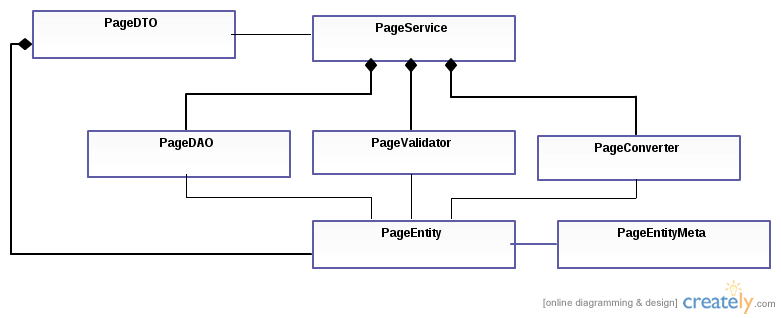
\includegraphics[width=5in]{figures/cms-uml.png}
\caption{Diagram tříd modelu}
\label{fig:modelUml}
\end{center}
\end{figure}

\subsection{Entity a metatřídy entit}
Entity z Datastore jsou v Javě reprezentovány doménovým modelem. Každé entitě odpovídá jedna třída s klíčem \verb|Key| a nastavenými třídními proměnnými jako parametry entity v uložišti. Tyto třídy jsou označeny anotacemi (například \verb|@Model|, \verb|@Attribute(primaryKey = true)|), jak bylo vidět na výpisech výše, což slouží ke generování metatříd. 

\subsection{DAO}
Ke každé entitní třídě je vygenerován jeden metaobjekt. Pro CRUD (Create, Read, Update, Delete) operace s entitou je vyhrazen speciální DAO objekt\footnote{Data Access Objekt - objekt zapouzdřující práci entitních tříd s databází}, každé entitní třídě odpovídá jeden DAO objekt. Máme zde veškerou práci s Datastore, pokud tedy budeme chtít změnit některé chování, máme tento kód na jednom místě a nemusíme procházet mnoho tříd. 

\subsection{Service}
S DAO třídami pracují takzvané servisní (Service) třídy. Znovu platí pravidlo, že servisní třídy odpovídají těm entitním. Jedná se vlastně o naše rozhraní do aplikace, protože MVC návrhový vzor počítá s nahraditelností všech částí, to znamená, že pokud bychom chtěli udělat z této aplikace místo webové desktopovou, stačilo by změnit Controller pro řízení vstupu a View pro zobrazování dat. Model by nepotřeboval žádnou změnu. Chybové stavy jsou do View předávány přes \verb|ServiceException|, která má navíc dvě specializované podtřídy \verb|ConverterException| a \verb|ValidatorException|, aby šlo jednoduše odlišit odkud chyba pochází. 

\subsection{Converter}
Servisní třída tedy používá třídy \verb|Converter| a \verb|Validator| odpovídaící entitám. Converter jak již název napovídá slouží ke konverzi vstupních parametrů od uživatele. Vše totiž do Controlleru aplikace přichází jako řetězec (\verb|String|) a tak je potřeba všechny položky převést na odpovídající typy a některé i podle speciálního nastavení, například datum podle určeného formátu na Javovský typ \verb|Date|. Converter se tedy postará o správné vytvoření entitní třídy podle vstupních pamatetrů anebo vyhodí výjimku s popisem chyby. 

\subsection{Validator}
Validační třída se pak postará o kontrolu entity, například zda textové pole nepřesáhlo maximální délku, anebo zda jsou vyplněna všechna pole, která nesmí být prázdná. S tímto nám také Slim3 pomáhá, máme zde již připravené některé běžné validátory (pro maximání délku řetězce, rozsah číselných hodnot anebo například kontrolu pomocí regulárních výrazů\footnote{Regulární výrazy (Regular Expression) - jedná se o speciální řetězec popisující množinu řetězců sloužící k vyhledávání nebo mainupulaci s textem}). Validátory navíc používají vygenerované metatřídy, abychom mohli specifikovat položku, kterou chcme zkontrolovat. Ve validátoru se rozlišují dva stavy, zda je vytvářen nový objekt, nebo zda jde jen o úpravu existující entity. To se používá například pokud chceme mít unikátní název URL pro stránku, aby systém věděl, kterou stránku má správně zobrazit. Při vytváření zkontrolujeme, zda již stejná URL neexistuje a při úpravě kontrolujeme, zda byla URL změněna, a poté zda nekoliduje s některou z existujících URL. 

\subsection{DTO}
Poslední důležitou vrstvou jsou DTO\footnote{Data Trasnfer Object - objekty sloužící pro transport entitních a dalších tříd}, ty slouží pro přenos entitních tříd mezi vrstvami Model a View. Jedná se o opak Converterů, pokud chceme zobrazit entitu uživateli, tak ji obalíme DTO objektem a ten se postará o správné převedení typů. Například datový typ \verb|Date| se podle nastavení převede do správného formátu data pro uživatele. 

\section{Propojení modelu - Google Guice}
Ke spojení všech těchto vrstev jsem se rozhodnul pro použití Google Guice\footnote{ http://code.google.com/p/google-guice/}. Jedná se o knihovnu pro Dependency Injection (injekce závislostí), kde můžeme pomocí anotace \verb|@Inject| nastavit přiřazení konkrétní implementace do třídních proměnných pomocí typu proměnné.

\begin{lstlisting}[caption={Ukázka použití Google Guice za pomocí anotace @Inject},label=lst:guiceInject,belowcaptionskip=0.4cm]
public class PageService {
	@Inject
	private PageDAO pageDAO;

	// ...
}
\end{lstlisting}

Výhodou nastavení rozhraní oproti přesnému určení typu třídy, je možnost měnit injektované třídy podle potřeby, například v jednom případě pro produkční prostředí a jinou implementaci pro testování, kde nastavíme například jen mock objekty\footnote{Mock objekty jsou simulované objekty, které napodobují reálné objekty používané hlavně při testování}. Pokud existuje v projektu jediná implemetace rozhraní, Guice ji najde a pomocí reflexe ji do proměnné nastaví. Pokud aplikace obsahuje více implementací daného rozhraní, musíme použít konfiguraci, kde nastavíme která implementace se má do proměnné nastavit. Konfigurace vypadá následovně:

\begin{lstlisting}[caption={Příklad konfigurace Google Guice},label=lst:guiceConfiguration,belowcaptionskip=0.4cm]
public class GuiceModule extends AbstractModule {
	public void configure() {
		bind(PageDAO.class).to(PageDAOImpl.class);
	}
}
\end{lstlisting}

Vše se nastavuje v jazyce Java, jen vybereme s jakou třídou má být rozhraní spojeno a takto vzniklou třídu předáme jako parametr při vytváření metodě \verb|createInjector|. Vytváření instancí objektu s nastavenými závislostmi pomocí Guice se provádí následujícím způsobem

\begin{lstlisting}[caption={Získávání sestavených tříd pomocí Google Guice},label=lst:guiceGetClass,belowcaptionskip=0.4cm]
Injector injector = Guice.createInjector(new BillingModule());
PageService pageService = injector.getInstance(PageService.class);
\end{lstlisting}

Výsledkem je instance třídy \verb|PageService| se správně nastavenými všemi závislostmi podle konfigurace. Pokud některý z nastavovaných objektů  také obsahuje závislosti označené pomocí \verb|@Inject| nastaví se také.

Výhoda Google Guice je, že jeho kód je poměrně malý v porovnání s ostatními knihovnami, které obsahují stejnou funkčnost. Guice se stará čistě jen o nastavení závislostí, kdežto například Spring framework a podobné se starají i o řešení dalších záležitostí. Proto je Guice vhodné použít na App Engine, nebude tak zdržovat načítání naší aplikace a závislost komponent v naší aplikaci bude nastavena na jednom místě.

\section{Slim3 Controller}
Slim3 nám kromě ulehčení práce s Datastore pomáhá i v Controller vrstvě návrhového vzoru MVC. Tato část se stará o řízení požadavků od uživatele, to znamená, že pokud navštíví určitou URL adresu, tak framework přesměruje požadavek do správného controlleru. Překlad funguje následujícím způsobem: pokud navštívíme základní URL \verb|/|, použije se třída \verb|IndexController| ze základního javovského balíčku (package) aplikace. Pokud navštívíme konkrétní stánku, například \verb|/page|, použije se třída \verb|PageController| ze základního balíčku. Dále pokud navštívíme podstránku \verb|/page/subpage| použije se třída \verb|SubpageController|  (tedy první písmeno je velké, jak je u tříd v Javě zvykem, a přidá se \verb|Controller|) z balíku \verb|page| a tak dále, můžeme do sebe vnořovat libovolný počet balíků a vždy když bude URL končit \verb|/| použije se \verb|IndexController| aktuálního balíku. 

Dalším vylepšením je možnost konvertovat parametry URL na GET\footnote{GET je parametr HTTP protokolu, kde se proměnné přenášejí v URL, například: url?klic=hodnota\&klic2=hodnota2} parametry zpracovatelné pomocí \verb|request.getParameter|. Vše se konfiguruje ve třídě \verb|AppRouter| následujícím způsobem:

\begin{lstlisting}[caption={Konfigurace nastaveníURL},label=lst:urlConfiguration,belowcaptionskip=0.4cm]
public class AppRouter extends RouterImpl {
	public AppRouter() {
		addRouting("/edit/{key}/{version}", 
			"/edit?key={key}&version={version}");
	}
}
\end{lstlisting}

URL \verb|/edit/xxx/1| se převede na \verb|/edit?key=xxx&version=1|, použije se tedy \verb|EditController| a v parametrech objektu \verb|Request| bude: \verb|key=xxx| a \verb|version=1|. \verb|EditController| je pak obyčejná třída dědící od třídy \verb|Controller|, kde přepíšeme metodu \verb|runBare()| s naší požadovanou funkčností. Máme zde dostupné všechny objekty jako máme k dispozici v servletu\footnote{Servlet je komponenta napsaná v jazyce Java, určená pro spouštění na webovém serveru}, jsou zde tedy dostupné objeky: \verb|Request|, \verb|Response| i \verb|ServletContext|.

U této vrstvy bylo důležité zajistit, aby webové uživatelské rozhraní správně zpracovávalo vstup od uživatele a také, aby aplikace správně informovala uživatele o nastalých akcích, jako jsou vložení stránky nebo chyba při validaci vstupu. Důležitým požadavkem bylo, aby byl uživatel informován i při přesměrování na jinou stránku (například po úspěšné akci) a aby byla zpráva zobrazena pouze jednou. Toto jsem vyřešil předáváním zpráv pomocí Session\footnote{Session umožňují identifikovat a rozeznat jednotlivé klienty při přechodu a přesměrování webových stránek}, pokud se má zobrazit po přesměrování. Aby se zpráva zobrazila pouze jednou, používá se trik, kdy se všechny zprávy předají do parametru objektu \verb|Request|, kam se ukládají informační zprávy, pokud nepotřebujeme uživatele přesměrovat. Vše je implementováno pomocí \verb|FlashScopeFiltru|\footnote{Filtry jsou standardni součástí webové Javy, kdy můžeme transformovat jednotlivé příchozí požadavky a odchozí odpovědi}, který je zařazen před \verb|FrontController|, kde se přesun zpráv do objektu \verb|Request| provede.

Pomocí připravených controllerů je vytvořena administrační část, kde jsou všechny URL adresy pevně dané a nebudou se měnit. Pro veřejnou část stránek, které jsou dynamicky generované uživateli aplikace, se používá třída \verb|IndexController|. Ta podle URL adresy vybere stránku z Datastore a získá všechny související entity, jako šablonu, štítky a další. Ze všech těchto dat nakonec naplní šablonu, sestaví stránku a tu odešle klientovi. Pokud se nepodaří stránku najít, tak přesměruje řízení na \verb|NotFoundController|, ten zobrazí zprávu o tom, že stránka nebyla nalezena a odešle chybový HTTP kód 404\footnote{HTTP stavový kód 404 podle dohody oznamuje klientovi, že stránka kterou požaduje, nebyla na serveru nalezena, to může být užitečné například pro vyhledávače, aby stránku nezařazovaly do svých výsledků}.

\section{View vrstva}
Poslední vrstva je View (neboli prezentační), která slouží k zobrazování webového obsahu uživatelům. Zde Slim3 používá klasické JSP\footnote{Java Server Pages - technologie umožňující generování webových stránek http://en.wikipedia.org/wiki/JavaServer\_Pages}, kde nám přidává několik značek (\emph{tagů}) pro usnadnění vykreslování formulářů a údajů z Datastore. JSP bylo vybráno pravděpodobně z toho důvodu, že je velmi rozšířené a je standardní součástí App Engine. JSP je vcelku jednoduché. Do HTML stránky přidáváme speciální tagy, které se zpracují. Můžeme také vytvářet vlastní knihovny tagů, které pak v JSP můžeme použí.

\section{Shrnutí implementace}
Struktura celé aplikace využívá návrhový vzor Model-View-Controller, kde jsou všechny části odděleny a mohou být jednoduše nahrazeny jinou implementací. Největší oporou při implementaci celé aplikace byl framework Slim3, který je vyvíjený přímo pro nasazení na cloudu App Engine. Tento framework nejvíce usnadňuje práci s modelem, umožňuje pracovat s relacemi mezi entitami. Framework nám usnadňuje i práci s controllery. Stará se o přesměrování požadavku na správný controller a řídí předávání informací od klienta. V prezentační vrstvě je využito technologie JSP a používají se speciální tagy pro zjednodušení zobrazení formulářů. K propojení vrstev v modelu je použita knihovna Google Guice sloužící k injektování závislostí pomocí speciálních anotací. Pro celkový návrh aplikace byla klíčová oddělenost, znovupoužitelnost a nahraditelnost všech částí. Aplikace je se pak stává libovolně rozšiřitelnou, lehce upravovatelnou a také jednoduše testovatelnou.